\documentclass[a4paper,dvipdfm]{article}
\usepackage[margin=1.1in]{geometry}
\usepackage[utf8]{inputenc}
\usepackage[brazil]{babel}
\usepackage{indentfirst}
\usepackage{cite}
\usepackage{url}
\usepackage{graphics}
\usepackage{graphicx}
\usepackage{caption}
\usepackage{subcaption}
\usepackage[acronym]{glossaries}
\usepackage{array}
\usepackage{multirow}
	

\title{Como o spam afeta a comodidade do Correio Eletrônico}
\author{Bianca Madoka Shimizu Oe\\
		Gustavo Shinji Inoue\\
		Rafael Umino Nakanishi}

\makeglossaries

\newglossaryentry{acm} {
	name={ACM},
	description={Association for Computing Machinery}
}
\newglossaryentry{blacklist} {
	name={\emph{blacklist}}, 
	description={Lista de mensagens classificadas como spam}
}
\newglossaryentry{bot} {
	name={\emph{bot}}, 
	description={Softwares criados para realizar alguma tarefa de forma automatizada}
}
\newglossaryentry{cabecalho} {
	name={cabeçalho}, 
	description={Parte do e-mail que contem informações suplementares de transmissão. Entre seus campos, são encontrados endereço do emissor, endereço do receptor, endereço de resposta, data de emissão, tipo do conteúdo e assunto}
}
\newglossaryentry{cadmarkov} {
	name={Cadeia de Markov},
	description={Conjunto de estados no qual um processo ocorre. O processo inicia em um estado e se move sucessivamente, transicionando entre estados a cada passo. O estado para o qual o processo se move depende unicamente, de forma probabilística, do estado em que ele se encontra atualmente},
	plural={Cadeias de Markov}
}
\newglossaryentry{captcha} {
	name={CAPTCHA}, 
	description={\emph{Completely Automated Public Turing test to tell Computers and Humans Apart}. Teste criado para diferenciar seres humanos de máquinas. Consiste em imagens de mensagens distorcidas para evitar a interpretação automática por máquinas}
}
\newglossaryentry{crm114} {
	name=\emph{CRM114}, 
	description={Software anti-spam baseado em técnicas estatísticas para a filtragem e classificação de dados. Seu código fonte na linguagem C é disponibilizado sob a licença \emph{GPL}}
}
\newglossaryentry{email} {
	name={e-mail}, 
	description={Correio eletrônico, termo usualmente utilizado para denotar a mensagem eviada por este meio}
}
\newglossaryentry{falsopos} {
	name={falso-positivo}, 
	description={Classificação errônea na qual, para este contexto, um e-mail legítimo é classificado como spam}
}
\newglossaryentry{OCR} {
	name={OCR},
	description={\emph{Optical Character Recognition}. Tecnologia criada para reconhecer caracteres a partir de uma imagem. Utilizado na digitalização de livros}
}
\newglossaryentry{gpl} {
	name={GPL}, 
	description={\emph{General Public License}. Licença para software livre}
}
\newglossaryentry{link} {
	name=\emph{link},
	description={Conexão que leva de uma página da \emph{Web} a, possivelmente, outra}
}
\newglossaryentry{listserv} {
	name=\emph{listserv},
	description={Softwares que permitem a inserção de endereços de e-mail em uma lista e o envio de e-mails para a lista de forma transparente}
}
\newglossaryentry{malware} {
	name={\emph{malware}},
	description={\emph{Malicious Software}. Software destinado a infectar um sistema, com o intuito de causar algum dano ou roubar informações}
}
\newglossaryentry{mime} {
	name={MIME},
	description={\emph{Multipurpose Internet Mail Extensions}. Padrão que define os tipos de mídia utilizados na Internet e extende o formato do e-mail para aceitar, entre outros, recursos multimídia}
}
\newglossaryentry{mta} {
	name={MTA},
	description={Mail Transfer Agent. Software que transfere mensagens de correio eletrônico de um cliente para outro, baseado em uma arquitetura cliente-servidor}
}
\newglossaryentry{oem} {
	name={software OEM},
	description={Produtos ou componentes comprados em grandes lotes a preços menores sob o nome de uma empresa}
}
\newglossaryentry{redezumbi} {
	name={rede zumbi},
	description={Rede formada por máquinas infectadas por malwares, geralmente destinada a enviar e-mails maliciosos ou contendo propaganda(\glspl{spambot})},
	plural={redes zumbi}
}
\newglossaryentry{spambot} {
	name=\emph{spambot},
	description={\Gls{bot} projetado para enviar spam de forma massiva, automaticamente}
}
\newglossaryentry{spammer} {
	name=\emph{spammer},
	description={Emissor de spam}
}
\newglossaryentry{threshold} {
	name=\emph{threshold}, 
	description={Valor utilizado como limitante para uma classificação}
}
\newglossaryentry{trigger} {
	name=\emph{trigger},
	description={Mecanismo executado ao ser acionado por um evento. Também chamado de ``gatilho''}
}
\newglossaryentry{whitelist} {
	name=\emph{whitelist}, 
	description={Lista de endereços de e-mail de remetentes legítimos, previamente validados}
}

\newcolumntype{C}[1]{>{\centering\let\newline\\\arraybackslash\hspace{0pt}}m{#1}}

\begin{document}

\begin{titlepage}
	\begin{center}
		\textsc{\huge Universidade de São Paulo}\\[0.3cm]
		\textsc{\Large Instituto de Ciências Matemáticas e Computação}\\[0.5cm]
		\textsc{\large SCC0207 - Computadores e Sociedade}\\[2.5in]
	
		\rule{\linewidth}{0.5mm} \\[0.7cm]
		{ \huge \bfseries Como o Spam afeta a comodidade do correio eletônico}\\[0.6cm]
		\rule{\linewidth}{0.5mm}\\[3in]

		{\large Bianca Madoka Shimizu Oe\\
		Gustavo Shinji Inoue\\
		Rafael Umino Nakanishi\\}

	\vfill
	\today
	\end{center}
\end{titlepage}

\newpage

\begin{abstract}
	O uso do correio eletrônico se tornou uma necessidade pessoal com o advento da tecnologia. Com esse novo meio de comunicação há maior praticidade e agilidade na troca de mensagens, de forma que não é necessário se locomover longas distâncias para conversar com outras pessoas.

	Entretanto, a facilidade adquirida também permite o envio de milhares de mensagens eletrônicas em poucos segundos, que podem ser mensagens importantes, como um aviso de uma empresa de grande porte para seus funcionários, ou \emph{spam}, um fenômeno que cresce cada vez mais.

	Nosso objetivo, nesta monografia, é mostrar como o spam vem trazendo inconveniências para usuários de \gls{email}.
	Mostraremos a origem da palavra e seus usos nos dias atuais, sua situação no mundo e estatísticas.
	Depois, apresentaremos métodos utilizados por provedores de e-mail para separar mensagens importantes de spam.
	Em seguida, alguns exemplos de como esse tipo de mensagem traz desconforto para quem o recebe. 
	Por fim, um estudo de caso, analisando as violações dos códigos da \gls{acm}~\cite{acm} e a conclusão.
	
	Os termos desconhecidos podem ter seus significados buscados no glossário, presente no fim desta monografia.
\end{abstract}

\newpage

\tableofcontents
\newpage

\section{Introdução}
	Nesta seção será feita uma breve descrição de como a palavra ``spam'' começou a ser utilizada para descrever e-mails indesejados.
	Em seguida, serão apresentados alguns fatos relacionados a este tipo de mensagem, considerando o Brasil e o mundo.

	\subsection{Origem do termo}
		A aparição da palavra Spam, que originou sua utilização atual, ocorreu no episódio 12 da segunda temporada de uma série britânica de comédia chamada \emph{Monty Python's Flying Circus}~\cite{montyPython:fc, mpyt}. 
		Spam é uma mistura de carnes de porco condimentadas e enlatadas, vindo de \emph{SPiced hAM} (Figura \ref{fig:spam}), criada pela empresa estadunidense \emph{Hormel Foods Corporation}.

		Durante o episódio, personagens discutem sobre o cardápio de um café. 
		A carne enlatada é um ingrediente presente em todos os pratos do estabelecimento, sendo considerada algo indesejável por um dos personagens. 
		Durante a discussão, ``Spam'' foi dito mais de 50 vezes em menos de 4 minutos.

		Apesar de não se saber ao certo quando o termo começou a ser utilizado para denotar mensagens indesejadas, atualmente ele é vastamente utilizado, principalmente para  se referir a e-mails de propagandas inconvenientes.
		
		\begin{figure}[ht]
			\centering
			
\includegraphics [height=5cm]{Imagens/spam/spam.png}
			\caption{Lata de presunto apimentado}
			\label{fig:spam}
		\end{figure}

	\subsection{Spam no mundo}
		A partir desta subseção, o termo spam será usado para denotar e-mail indesejado.
		
		A empresa especializada em segurança \emph{M86 Security Labs} separa spam em 13 categorias listadas abaixo~\cite{spam:m86-type}:
		\begin{description}
			\item [Fraude] Seu objetivo é fazer o destinatário acreditar que ganhou algo, como um prêmio.
			\item [Adulto] Possui conteúdo pornográfico e oferece cadastro gratuito a \emph{sites} adultos ou a serviços de acompanhantes.
			\item [Financeiro] É relacionado a financiamentos e oferecimento de crédito falso.
			\item [Ações] Anuncia ações de empresas para causar o aumento do preço das mesmas.
			\item [Farmacêuticas] Informa sobre vários tipos de drogas e remédios, geralmente promete uma pele melhor, mais energia, perda de peso, entre outros. 
			Como um exemplo, tem-se o Viagra.
			\item [Phishing] Tenta imitar e-mails legítimos enviados por empresas para conseguir dados e/ou credenciais de seus clientes.
			Seus alvos mais populares são bancos, \emph{eBay} e \emph{PayPal}.
			\item [Diplomas] Anuncia qualificações como diplomas de universidades ou cursos de treinamento.
			\item [Réplicas] Anuncia imitações baratas de produtos como bolsas, relógios e celulares.
			\item [Software] Anuncia softwares baratos, usualmente prometendo venda de \gls{oem}.
			\item [Malware] Contem anexos maliciosos ou \glspl{link} que levam a \emph{websites} com vírus.
			\item [Jogos de azar] Promove cassinos ou \emph{sites} de pôquer, que geralmente oferecem bônus por cadastramento.
			\item [Relacionamento] Podem ser incluídos na categoria de fraudes, em que mulheres ou homens que fingem ser mulher tentam criar um relacionamento para extorquir dinheiro.
			\item [Outros] Não são classificados nas categorias supracitadas.
		\end{description}

		A Figura \ref{fig:spamtype} mostra a distribuição do spam nas categorias descritas acima.

		\begin{figure}
			\centering
			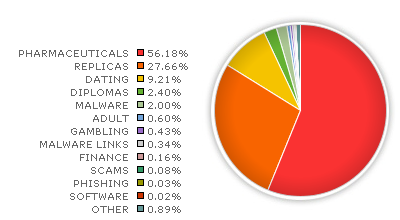
\includegraphics [height=5cm] {Imagens/m86security/spamtype.png}
			\caption {Distribuição do conteúdo de spam}
			\label{fig:spamtype}
		\end{figure}

		A distribuição de emissores de spam pelo mundo e pelo Brasil podem ser vistas na Figura \ref{fig:spamworld} e na Figura \ref{fig:spambrasil}, respectivamente.

	\begin{figure}[ht]
		\begin{subfigure}[b]{\textwidth}
			\centering
			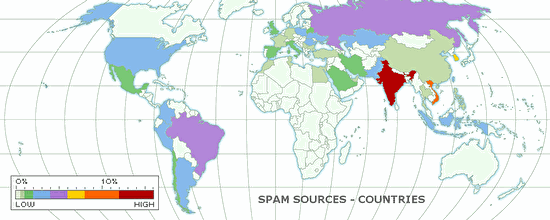
\includegraphics[height=5cm]{Imagens/m86security/spam-country-map.png}
			\caption{Mapa-múndi de emissores de spam. Cores mais escuras indicam maior emissão.}
		\end{subfigure}
		~
		\begin{subfigure}[b]{0.47\textwidth}
			\centering
			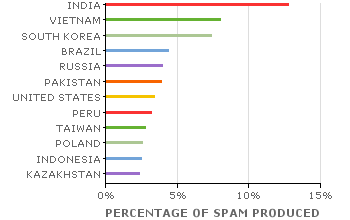
\includegraphics[height=5cm]{Imagens/m86security/spam-country-bar.png}
			\caption{12 países que mais emitem spam}
		\end{subfigure}
		~
		\begin{subfigure}[b]{0.47\textwidth}
			\centering
			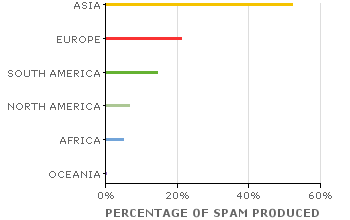
\includegraphics[height=5cm]{Imagens/m86security/spam-continent-bar.png}
			\caption{Percentual de spam emitido por continente}
		\end{subfigure}
		\caption{Emissão de spam no mundo}
		\label{fig:spamworld}
	\end{figure}
		~
	\begin{figure}
		\centering
		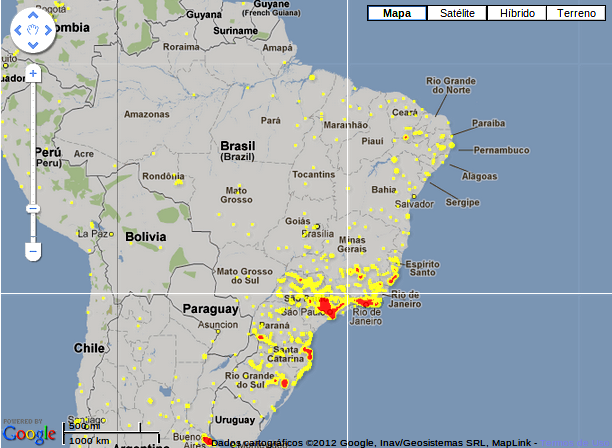
\includegraphics[height=7cm]{Imagens/spam/brasilspam.png}
		\caption{Focos de emissores de spam no Brasil}
		\label{fig:spambrasil}
	\end{figure}
	
	Como se pode ver, no Brasil, os estados que mais emitem spam são o estado de São Paulo e o Rio de Janeiro, o que condiz com o fato de que são os pólos tecnológicos do país.

	Já no âmbito global, a regra não pode ser generalizada, por ser uma questão que não depende somente do aspecto tecnológico, mas também do econômico e cultural.

	Pode-se tomar como exemplo a Índia, que segundo o mapa da empresa M86 Security Labs e de outra empresa de segurança chamada Sophos~\cite{sophos} é o país que mais envia mensagens ilegítimas no mundo.
	O grande aumento na quantidade de spam produzido foi, em parte, causado pela expansão rápida de redes com acesso à Internet no país.

	Segundo um consultor na Sophos, a inexperiência de muitos usuários de primeira viagem os levou a serem vítimas de criminosos virtuais, pois a maioria não toma medidas para bloquear infecções por \gls{malware}, adicionando seus computadores a enormes \glspl{redezumbi}~\cite{spam:india}, que acarreta no aumento das mensagens enviadas. 

\newpage
\section {Estatísticas}
	Nesta seção são mostrados dados estatísticos sobre o percentual de spam e seu crescimento nos últimos anos, assim como algumas curiosidades.
	
	\vspace{10pt}
	\begin{enumerate}
		\item
			Na Figura \ref{fig:spambar} estão contidos dados sobre a quantidade de spam, dividida nas categorias abaixo para o ano fiscal de 2011 a 2012~\cite{spam:stats}.
		\begin{itemize}
			\item Spam confirmado, representado nos gráficos como \emph{Positive Spam};
			\item Mensagem suspeita, representada nos gráficos \emph{Suspected Spam};
			\item Mensagen legítima, representada nos gráficos como \emph{Legitimate Messages};
			\item Marketing.
		\end{itemize}
	
		\begin{figure}[h!]
			\centering
			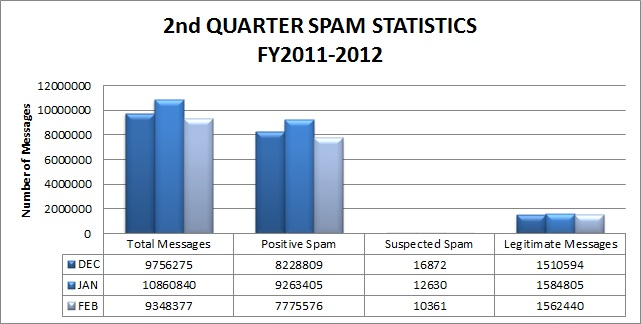
\includegraphics[height=7cm]{Imagens/spam/2ndQtr-FY2011-12.jpg}
			\caption{Quantidade de spam de 2011 a 2012}
			\label{fig:spambar}
		\end{figure}
	
	\item
		Em abril de 2012, o sistema antispam \emph{IronPort Antispam System} processou 14.856.078 mensagens de e-mail, das quais 13.158.245 foram identificadas como spam, 10.151 foram classificadas como suspeitas e 419.407 como marketing, acumulando um total de 13.168.396 ($88.6\%$) de spam~\cite{spam:stats}.
		Os dados podem ser visualizados no gráfico da Figura \ref{fig:spampizza}.
	
		\begin{figure}[h!]
			\centering
			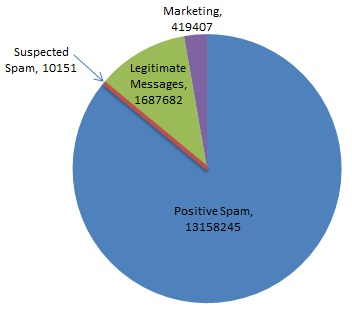
\includegraphics[width=7cm]{Imagens/spam/Apr2012-Spam.jpg}
			\caption{Quantidade de spam nas mensagens processadas em abril}
			\label{fig:spampizza}
		\end{figure}
	
	\item
		Foi feito um experimento com os softwares antispam \emph{Cloudmark}~\cite{cloudmark}, \emph{Barracuda}~\cite{barracuda} e \emph{SpamAssassin}~\cite{spamassassin} para descobrir quais são os \glspl{trigger} mais comuns para os filtros de spam dos programas supracitados~\cite{spam:trigger}.
		Alguns dos resultados obtidos são mostrados abaixo.
		\begin{itemize}
			\item Mensagem possui pouco texto em comparação à área ocupada por imagens;
			\item Mensagem só possui tipos \gls{mime};
			\item Assunto está completamente em maiúsculo;
			\item Utilização da frase ``extra inches'', traduzida como ``polegadas extra'';
			\item Utilização da frase ``You registered with a partner'', traduzida como ``Você se registrou com um companheiro''.
		\end{itemize}
	
	\item
		As palavras mais frequentes em mensagem de spam, segundo a empresa de segurança \emph{Symantec}, dependem do \emph{spambot} que envia a mensagem, já que cada um tem uma função específica~\cite{spam:words}.
		Algumas dessas palavras podem ser vistas nas Figura \ref{fig:wordlist}.
	
		\begin{figure}[h!]
			\centering
			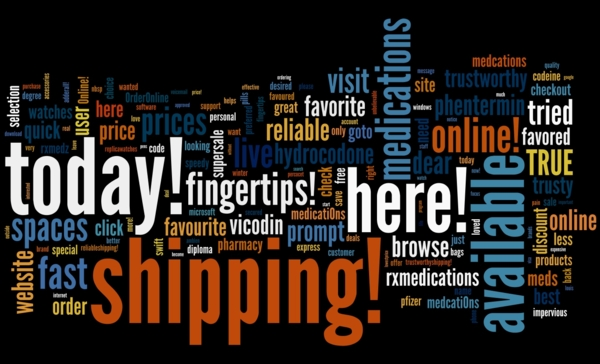
\includegraphics[height=7cm]{Imagens/spam/words-shipping.jpg}
			\caption{Palavras populares em spam}
			\label{fig:wordlist}
		\end{figure}
	
		Como se pode perceber, é comum a utilização do ponto de exclamação, pois, segundo Daren Lewis, empregado da empresa, os \glspl{spammer} criam uma sensação de urgência na mensagem, já que quanto menos tempo pessoas pensam sobre o que está escrito, menos elas percebem que é uma farsa.
	\end{enumerate}
	
\newpage

\section{Filtros de Spam}
	Para acompanhar o aumento do número e da variedade de spams, vem sendo criados vários métodos para separar mensagens importantes de propagandas.
	São inúmeras as abordagens utilizadas. 
	Algumas se baseiam no \gls{cabecalho} da mensagem, outras na frequência das palavras utilizadas.
	Nas seções seguintes, serão brevemente discutidas algumas estratégias utilizadas no combate ao spam, e, como um exemplo, serão mostrados alguns dos filtros utilizados pelo \emph{Gmail}~\cite{filtros, gmail:youtube, gmail:fightspam}.

	\subsection{Filtro baseado na estrutura do texto}
		Este tipo de filtro se baseia em cadeias específicas do cabeçalho do e-mail, como, por exemplo, a língua na qual foi escrito e o tipo do conteúdo da mensagem.

		Estes filtros são utilizados pela grande maioria dos provedores do serviço de correio eletrônico e de softwares criados para filtrar mensagens.

		Sua grande vantagem é não precisar de dados de alto nível, como a informação semântica da mensagem, para poder separar os e-mails.

		Deve ser tomado um certo cuidado em relação a este filtro, pois, como foi mostrado na seção anterior, alguns dos métodos utilizados para este tipo de filtragem são subjetivos, como, por exemplo, a taxa entre imagens e texto.
		Por isso, ele deve ser utilizado em conjunto com outros tipos de filtros, que serão descritos a seguir.


	\subsection{\emph{Whitelist}/Verificação}
		Uma abordagem mais agressiva para a filtragem de spam é a utilização de \glspl{whitelist} em conjunto com a verificação automática.

		Qualquer endereço que esteja nesta \emph{whitelist} tem sua mensagem enviada sem maiores problemas.
		Se o endereço não estiver contido na lista, o \gls{mta} envia uma mensagem de volta para o remetente, com instruções que, ao serem seguidas, adicionam o endereço do remetente na \emph{whitelist}.

		Como a maioria das mensagens de spam possui endereços de resposta falsos, as instruções não seriam seguidas e o e-mail não chegaria à caixa de entrada do destinatário.
		Caso o \emph{spammer} decida fazer o que lhe foi dito, ele será adicionado à lista, porém isso o torna mais facilmente rastreável.
		
		Apesar de ser uma maneira eficaz de diminuir os spams, ela pode prejudicar usuários legítimos que não podem ou querem atender a essa exigência, já que isso implicaria no não recebimento de sua mensagem.
		Logo, a forma de validação do endereço deve ser ponderada para que não seja fácil demais, permitindo a validação automatizada, nem difícil demais, impedindo usuários legítimos de utilizarem o correio eletrônico.
		
		Como um exemplo deste tipo de abordagem, tem-se o \emph{Corlive.com}~\cite{corlive}, que é um servidor de e-mail que utiliza \gls{captcha}~\cite{captcha} para validar os e-mails enviados e não permitir que \emph{bots} enviem spam.

	\subsection{Distribuição adaptativa de \emph{blacklist}}
		A \gls{blacklist} é formada por mensagens que foram classificadas como spam por usuários ou por ``honeypots'', que são endereços especiamente criados por servidores para atrair spam.

		Ao receber uma mensagem, o MTA utiliza um filtro por \emph{blacklist} para determinar se mesma é um spam conhecido, e ela só é enviada à caixa de entrada do destinatário caso ela não seja classificada como ilegítima.

		Esta estratégia se baseia no uso de técnicas estatísticas para sumarizar o conteúdo de um mensagem de forma que pequenas mutações no spam não impeçam seu reconhecimento.

		A probabilidade de haver falsos-positivos é pequena, já que é necessária uma marcação na mensagem para que ela entre na \emph{blacklist}. Além disso, quando ocorre uma marcação errônea de mensagens vastamente enviadas, como informativos, o gerenciador da lista pode desmarcá-las.
		
		Como é necessária a verificação da mensagem em um servidor, a performance deste método comparada a outros é baixa, sendo ele bastante lento.

		Um exemplo de software que implementa esta abordagem é o \emph{Pyzor}~\cite{pyzor}, um software implementado em \emph{Python} sob a licença \gls{gpl}.

	\subsection{Ranking baseado em regras}
		Este filtro possui regras para pontuar mensagens, que são formadas principalmente por expressões regulares, e tenta fazer correspondências entre o padrão e a mensagem.
		Cada equivalência adiciona ou diminui pontos da mensagem, que são guardados para posterior avaliação.
		
		Se a quantidade de pontos do e-mail exceder um determinado \gls{threshold}, a mensagem é classificada como spam, caso contrário, é classificada como legítima.

		A dificuldade deste tipo de filtro é que, apesar de existirem regras que são constantes com o decorrer do tempo, como checar se o endereço de resposta é falso ou possuir áudio como tipo de conteúdo, há outras que mudam com o tempo, como os produtos dos quais os spams fazem propaganda, o que causa a necessidade constante de atualização das regras.

		Um software que implementa este tipo de filtro é o \emph{SpamAssassin}~\cite{spamassassin}, um projeto open-source da \emph{Apache}.

	\subsection{Filtro Bayesiano}
		A abordagem do filtro Bayesiano, criado por Paul Graham~\cite{bayes:graham}, é a utilização de modelos Bayesianos de probabilidade para determinar se uma mensagem é legítima ou não.

		É criado um dicionário de palavras contendo a probabilidade de ela estar em um spam e a probabilidade de estar em uma mensagem válida. Esse dicionário é utilizado para calcular a probabilidade geral de a mensagem ser um spam, com base na teoria da probabilidade condicional de Bayes.

		Este filtro possui traz vários benefícios como ser automatizável, ou seja, não são necessárias pessoas para definir os valores de probabilidade, já que ele pode aprender, isto é, adicionar novas palavras ou modificar a probabilidade de uma palavra de acordo com a marcação de um e-mail como spam ou válido.

		Além disso, sua implementação e a teoria em que se baseia são extremamente simples e sua performance, em geral, é melhor que a de filtros baseados em regras.
		
		Um software que implementa o filtro Bayesiano é o \emph{SpamBayes}~\cite{spambayes}, disponível para os serviços de e-mail \emph{Gmail}, \emph{MSN Hotmail}, \emph{Yahoo! Mail}, entre outros.

	\subsection{Filtro Markoviano}
		O filtro Markoviano é um filtro estatístico baseado na teoria de \glspl{cadmarkov}~\cite{markov}, e leva em consideração a probabilidade de transição entre uma palavra e outra, ou seja, dada uma palavra, ele tenta predizer qual é a próxima.

		Diferentemente do filtro Bayesiano, que é baseado na probabilidade de ocorrência de palavras independentes, o filtro Markoviano trabalha em cima de frases, e por isso, seu desempenho tende a ser maior, já que utiliza uma abordagem holística do texto.
		
	Esta estratégia é utilizada no filtro de spam \gls{crm114}~\cite{crm114}, juntamente com outras abordagens que não serão discutidas nesta monografia. Seu desempenho foi testado para diferenciar documentos japoneses confidenciais de não confidenciais, e a acurácia obtida foi maior que $99\%$ e taxa de falsos-positivos foi menor que $5.3\%$~\cite{fmarkov:japtest}.

	\subsection{Gmail}
		Uma das técnicas utilizadas pelo provedor de serviço de correio eletrônico \emph{Gmail} é o aprendizado baseado em instâncias, chamado pelo provedor de \emph{Community clicks}, em que os filtros de spam usados para todos os usuários são modificados a cada mensagem que um usuário marca como spam ou como mensagem legítima~\cite{gmail:fightspam}.

		Outra técnica é o aprendizado de máquina usado para combinar e indexar os conjuntos de busca do buscador Google, que permite a junção de vários fatores para identificar mensagens semelhantes e classificá-las como spam, como um filtro por distribuição de blacklist.
		
		Além disso, são aplicadas ferramentas como \gls{OCR} de outro serviço da empresa, o \emph{Google Book Search}, serviço de busca em livros (podem ser imagens), para identificar spams em forma de imagens~\cite{gmail:youtube}.

		A filtragem pode feita por endereço, ou seja, se um usuário marca a mensagem de um emissor como spam várias vezes, próximas mensagens enviadas por esse endereço irão para a caixa de spam automaticamente.

		Em conjunto, sempre é checado se o endereço do remetente é autenticado por meio de órgãos autenticadores para tentar impedir golpes de \emph{phishing}.
		Entretanto, não ter um certificado não é suficiente para a mensagem ser marcada como spam.
		Esta checagem é feita como parte da filtragem e é combinada com denúncias de usuários e outras técnicas~\cite{gmail:filtros}.

		O \emph{Gmail} também permite a criação personalizada de fitros de spam baseados em regras, de acordo com os seguintes campos do e-mail: remetente, destinatário, assunto e corpo da mensagem. 
		É possível, ainda, filtrar pela presença ou ausência de palavras, utilizar operadores lógicos como \emph{e}, \emph{ou} e \emph{não}, e denotar ``qualquer um'' por meio de ``\emph{*}''.

		Com todo esse leque de ferramentas, a filtragem feita pelo serviço de correio eletrônico do gigante buscador é bastante interessante e a melhora de sua eficácia pode ser vista na Figura \ref{gmail:chart}.

		\begin{figure*}[ht]
			\centering
			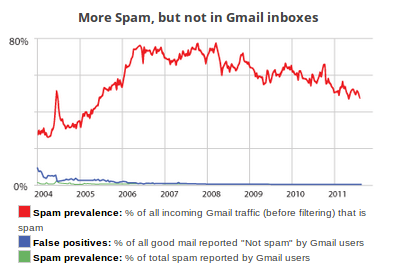
\includegraphics[height=7cm]{Imagens/gmail/spamchart.png}
			\caption{Percentual de filtragem ao longo dos anos}
			\label{gmail:chart}
		\end{figure*}

\newpage
\section{Casos Reais}
	Nas próximas subseções, são apresentados casos reais de como o spam afeta o cotidiano das pessoas.

	\subsection {Coxinha na promoção}
		A colunista Lúcia Guimarães do jornal Estado de São Paulo recebeu uma notificação de uma promoção de uma coxinha bo Boteco do Joaquim, na Cidade Baixa em Porto Alegre.
		O salgado, um espeto de ``Coxinha de Asa'', custava $R\$12,50$ e, com um desconto de aproximadamente $50\%$, passou a custar $R\$6,00$.

		A notificação da promoção para Lúcia foi feita via e-mail e ela gostaria de aproveitar a promoção, se pudesse.
		O comentário feito por Lúcia sobre o e-mail pode ser visto à seguir~\cite{cr:coxinha}.

		\begin{quotation}
			Foi o Boteco do Joaquim que avisou esta guria da promoção. E concluo a afirmação no tom agudo de uma interrogação, como fazem os gaúchos. Uma pena que não posso economizar $R\$ 6,50$ num almoço porque a passagem daqui para o Boteco custa $R\$ 4$ mil.
		\end{quotation}

		Como se pode perceber, a escritora não mora em Porto Alegre.
		Na verdade, sua atual moradia é em Nova Iorque e, ainda assim, ela recebe e-mails com propagandas de coxinhas da Cidade Baixa.
		Esse não foi o único spam que recebeu com propagandas de lugares em que ela não poderia chegar, como se pode ver pelo trecho abaixo:

		\begin{quotation}
			Se alguma corporação estiver espionando minha correspondência eletrônica com base num algoritmo, pode montar um perfil em que: 
			Eu como coxinha em Porto Alegre; 
			corto o cabelo em Belo Horizonte; 
			compro câmeras no Estado do Maine; 
			passo os fins de semana em Búzios; 
			encomendo pornografia do Estado de Nevada. 
			Enfim, sou uma verdadeira cidadã do mundo, cheia de caprichos e perversões.
		\end{quotation}
			
		O que se pode concluir a partir deste caso é que o objetivo do Boteco do Joaquim foi atingido, já que a jornalista leu o e-mail e compraria a coxinha se conseguisse, porém a propaganda poderia ser enviada de forma mais inteligente somente para potenciais consumidores, categoria na qual Lúcia não se inclui.

	\subsection {Amizades via Spam}
		Um \emph{spammer} indiano enviou um \emph{e-mail} escrito em malaialo (idioma do estado de Kerala, no sul da Índia)
	que foi promovido por uma revista de notícias online chamada \url{gulfmalayaly.com}.

		O problema começou com um \emph{e-mail} de resposta automática da empresa \emph{Business Wire Inc.} que era programado
	para responder ao remetente original. No entanto, essa mensagem acabou sendo enviada a todas as pessoas que
	receberam o \emph{spam original}.

		A pedido do renomado \emph{Wall Street Journal}, a \emph{Google} analisou-o e chegou a
	conclusão de que isso se devia ao fato de elas terem sido automaticamente adicionadas a uma lista de \emph{e-mail}. Tal lista
	teria sido incluída na lista de destinatários.

		Poucos minutos depois, várias reclamações foram surgindo de várias partes do mundo. Eles reivindicam sua remoção da lista.
	Qualquer pessoa que clicasse em ``\emph{Reply All}'' acharia que estava mandando o que escreveu a uma minoria, quando na verdade ela 		estaria enviando-o à lista.

		Dentre os destinatários, estava o serviço de atendimento ao cliente do \emph{Starwood Hotels}. Uma representante da instituição,
	entendendo que as pessoas queriam ser removidas da lista de \emph{e-mails} do \emph{Starwood}, enviou educadamente uma observação. As
	pessoas que estavam na lista concluíram que o ataque teria sido originado no próprio \emph{Starwood Hotels}. No entanto, a \emph{Starwood} não estava respondendo mais.

		As reclamações continuaram até que Pádraig Belton, um escritor de Londres, sugeriu que todos se reunissem em um \emph{pub}.
	Tempos depois, Robert Peacock, um executivo empresarial em Londes, sugeriu que fosse estabelecido um elo entre eles. No dia
	seguinte, Andrew Wong criou o grupo \emph{Unified by Spam - The Social Experiment} ~\cite{ubs} no \emph{LinkedIn} (rede social para contatos
	profissionais), sendo que atualmente ele conta com aproximadamente 150 membros.

		Várias pessoas tomaram o acontecimento como gatilho para se relacionar com novas pessoas e conhecer novos países.~\cite{cr:ubs}

	\subsection {Hacker britânico invade privacidade}
        Em julho de 2006, em \emph{Drummuir} (Escócia), Matthew Anderson, 33 anos, foi
condenado a um ano e meio de
	prisão por invadir os computadores de outras pessoas.

	    A invasão era realizada através do envio de milhares de mensagens de
    \emph{spam} que continham vírus em seu conteúdo. Ao abri-lo, esse vírus se
    instalava no computador, garantindo ao \emph{hacker} acesso total aos arquivos de
dados e à \emph{webcam} das vítimas - espionando a casa das pessoas sem ser
reconhecido.

	    A Polícia Metropolitana de Londres descobriu que Anderson guardava
    imagens da casa das vítimas e cópia de documentos particulares como contas,
    relatórios médicos, currículos, listas de senhas e fotografias.
        Ele agia da sala da casa de sua mãe.

	O motivo da prisão foi modificação não-autorizada de sistemas de informática.

\newpage
\section{Estudo de Caso}
	O estudo de caso apresentado à seguir é baseado em fatos, mas não é completamente real. 

	\subsection{Contexto}	
    Juliano, professor de uma universidade renomada, ficou responsável por ministrar uma disciplina em um determinado semestre e delegou a tarefa de auxiliá-lo (como monitor bolsista) a Eduardo. 
	Eduardo, por sua vez, é pós-graduando sob a tutoria de Juliano e está na iminência de defender sua tese de mestrado.

    A média final da disciplina ministrada é composta por projetos (para serem feitos em grupos) de complexidade média e por nenhuma prova.
	Os projetos são lançados ao longo do semestre e cada um deles fica responsável por cobrir parte do conteúdo programático.

	Durante a realização do projeto, é necessário fazer vários testes para comprovar a eficiência da implementação escolhida para resolver o problema proposto. 
	Os testes devem ser feitos em máquinas específicas fornecidas pela instituição.
	
	Como as máquinas são compartilhadas por todos os grupos e ocorriam testes simultâneos, havia flutuações indesejadas nos resultados obtidos.
	Por isso, após várias reclamações, o professor decidiu alocar períodos de tempo reservados para cada grupo, de forma que outros grupos seriam penalizados caso utilizassem os recursos em um período que não fosse seu.

	Foi feita uma alocação inicial, escolhida por Juliano, porém os horários não levavam em conta a disponibilidade dos alunos. 
	Consequentemente, havia grupos que não estavam livres durante seu período, o que levou vários a enviarem e-mails ao professor para pedir que a alocação fosse modificada.
	Além disso, houve grupos que não conseguiram terminar seus testes na sua vez e pediram mais tempo para o professor.

	Juliano decidiu atender ao pedido dos alunos e disse para Eduardo mandar-lhes um e-mail para avisar-lhes sobre as mudanças feitas.
	
	Eduardo fez como lhe foi dito e enviou e-mails a todos os alunos matriculados na disciplina, avisando sobre as modificações e extensões nos horários.
	Entretanto, após alguns envios, percebeu que ainda aconteceriam várias modificações e que isso geraria uma grande quantidade de mensagens enviadas que não eram importantes para todos os alunos, como, por exemplo, os alunos que já haviam realizado os testes de forma bem sucedida.

	Era possível utilizar o \emph{site} da disciplina para avisar sobre as modificações, assim como foi feito para a primeira alocação. 
	O problema é que somente o professor poderia fazê-lo, e, quando Eduardo sugeriu esta possibilidade, Juliano não pareceu disposto a gastar seu tempo de pesquisa para atualizar o documento que continha os horários reservados.

	Havia, ainda, a possibilidade de enviar o aviso somente para os grupos influenciados pela modificação, mas isso seria mais trabalhoso do que a primeira opção, já que Juliano ou Eduardo teriam que escolher para quem mandariam a mensagem.
	
	Eduardo sabia que se mandasse os e-mails, vários alunos ficariam insatisfeitos e isso poderia ser considerado spam e alertou Juliano, que respondeu ser irrelevante.

	O orientando não queria irritar seu orientador às vésperas de sua defesa, já que isso poderia prejudicá-lo. 
	Por outro lado, se estivesse no lugar dos alunos, se sentiria incomodado pelo spam acadêmico recebido.

\newpage
	\subsection{Dados relevantes}
		No caso estudado, são as partes envolvidas são:
		\begin{itemize}
			\item Juliano
				\begin{itemize}
					\item Professor;
					\item Orientador de Eduardo;
					\item Pesquisador da universidade.
				\end{itemize}
			\item Eduardo
				\begin{itemize}
					\item Mestrando prestes a defender sua tese;
					\item Monitor da disciplina;
					\item Orientando de Juliano.
				\end{itemize} 
			\item Alunos
				\begin{itemize}
					\item Matriculados na disciplina ministrada por Juliano e monitorada por Eduardo;
					\item Insatisfeitos com a quantidade de e-mails recebidos. 
				\end{itemize}
		\end{itemize}

		As obrigações das partes envolvidas para com as outras são dadas na Tabela \ref{tab:obrig} e na Figura \ref{fig:obrig}.

		\begin{table}[h!]
			\centering
			\begin{tabular}{@{\extracolsep{\fill}}l C{0.15\textwidth} C{0.15\textwidth} C{0.15\textwidth}}
				\hline
									&	Juliano		&	Eduardo	&	Alunos\\	
				\hline
				Juliano	&	Pesquisar	&	Orientar para a docência	&	Passar conhecimento\\
				\hline
				Eduardo	&	Obedecer \linebreak \linebreak Auxiliar na disciplina	&	Prezar pela \linebreak pós-graduação	&	Avisar sobre \linebreak mudanças\\
				\hline
			Alunos	&	Ser aprovado na disciplina	&			&	Manter boas notas\\
				\hline
			\end{tabular}
			\caption {Tabela de obrigações}
			\label{tab:obrig}
		\end{table}
		~
		\begin{figure}[h!]
			\centering
			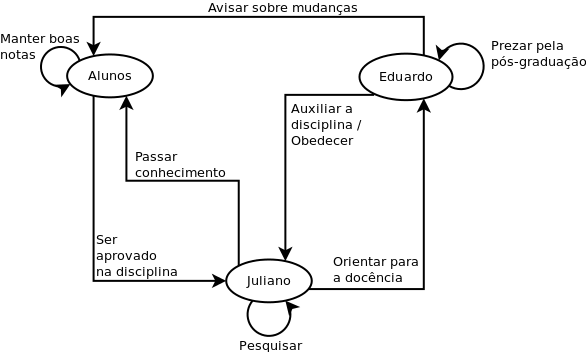
\includegraphics[height=7cm]{diagramas/grafo-de-obrigacoes.png}
			\caption{Grafo de obrigações}
			\label{fig:obrig}
		\end{figure}

		As alternativas de decisão de Eduardo são:
		\begin{itemize}
			\item Insistir para Juliano modificar o documento no \emph{site};
			\item Enviar e-mails sobre as modificações somente para os alunos influenciados pelas mudanças feitas (componentes dos grupos);
			\item Enviar e-mails de todas as modificações a todos os alunos matriculados;
			\item Guardar as modificações e enviá-las em blocos para todos os alunos.
		\end{itemize}
	
	\subsection{Códigos de ética da ACM violados}
		Os códigos da ACM violados são os seguintes:
		\begin{itemize}
			\item ``Contribuir para o bem-estar humano e da Sociedade''\\
				Se Eduardo enviar e-mails a todos os alunos sobre as modificações, os alunos não interessados se sentirão incomodados.
				Além disso, Juliano corre o risco de atribuir horários inconsistentes por não possuir todas as informações de forma organizada;
			\item ``Procurar alcançar a maior qualidade, eficácia de dignidade tanto nos processos como nos produtos do trabalho profissional''\\
				Se Eduardo enviar e-mails sobre as notificações, os alunos interessados, Eduardo e Juliano perderão tempo por ter que buscar as modificações em sua caixa de e-mail.
				Além disso, Juliano corre o risco de atribuir horários inconsistentes por não possuir todas as informações de forma organizada;
%			\item ``Adquirir e manter competência profissional''\\
%				((TODO))
				
		\end{itemize}

	\subsection{Potenciais benefícios e vulnerabilidades}
		Os potenciais benefícios de cada solução são dados na Tabela \ref{tab:ben} e as potenciais vulnerabilidades são dadas na Tabela \ref{tab:vul}.

		Os alunos foram divididos em dois grupos: alunos interessados e alunos não interessados.
		O primeiro grupo é composto pelos alunos relacionados às modificações, enquanto o segundo é composto pelos outros.
		\begin{table}[h!]
			\centering
			\begin{tabular}{@{\extracolsep{\fill}}C{0.15\textwidth}  C{0.15\textwidth} C{0.15\textwidth} C{0.15\textwidth} C{0.15\textwidth} C{0.15\textwidth}}
				\hline
				 & \textbf{Insistir para Juliano modificar no site} & \textbf{Enviar apenas para os interessados} & \textbf{Enviar para todos} & \textbf{Enviar blocos de modificações}\\
				\hline
				Alunos interessados & Não receberão nenhum e-mail \linebreak \linebreak Serão notificados & Serão notificados & Serão notificados & Receberão menos e-mails \linebreak \linebreak Serão notificados\\
				\hline
				Alunos não interessados & Não receberão nenhum spam & Não receberão nenhum spam &  & Receberão menos e-mails\\
				\hline
				Eduardo & Não precisa enviar os e-mails & & & Envia menos e-mails \\
				\hline
				Juliano & & Não envia e-mails & Não envia e-mails & Não envia e-mails \\
				\hline
			\end{tabular}
			\caption{Tabela de benefícios potenciais}
			\label{tab:ben}
		\end{table}
		~
		\begin{table}[h!]
			\centering
			\begin{tabular}{@{\extracolsep{\fill}}C{0.15\textwidth} C{0.15\textwidth} C{0.15\textwidth} C{0.15\textwidth} C{0.15\textwidth}}
				\hline
				& \textbf{Insistir para Juliano modificar o documento no site} & \textbf{Enviar apenas para os interessados} & \textbf{Enviar para todos} & \textbf{Enviar blocos de modificações}\\
				\hline
				Alunos interessados & & & Recebe spam & Recebe spam \\
				\hline
				Alunos não interessados & & & Recebe spam & Recebe spam \\
				\hline
				Eduardo & & Envia e-mails & Envia e-mails & Envia e-mails \\
				\hline
				Juliano & Precisa modificar o documento & & &\\
				\hline
			\end{tabular}
			\caption{Tabela de vulnerabilidades potenciais}
			\label{tab:vul}
		\end{table}
		~
		\begin{table}[h!]
			\begin{tabular*}{\textwidth}{@{\extracolsep{\fill}} C{0.117\textwidth} | C{0.117\textwidth} C{0.117\textwidth} C{0.117\textwidth} C{0.117\textwidth} C{0.117\textwidth} C{0.117\textwidth}}
				\cline{2-7}
				& & & \textbf{Insistir para Juliano modificar no site} & \textbf{Enviar apenas para os interessados} & \textbf{Enviar para todos} & \textbf{Enviar blocos de modificações}\\
				\hline
				\multirow{3}{*}{Eduardo}  & Para ele mesmo & Prezar pela pós-graduação & - - & - - & - & - \\
				\cline{2-7}
						& Juliano & Obedecer & - & + & + + & + \\
				\cline{2-7}
						& Alunos & Notificar & + - & + & + & + \\
				\hline
				Juliano & Para ele mesmo & Pesquisar & - - &  &  & \\
				\hline
			\end{tabular*}
			\caption{Tabela de obrigações afetadas}
		\end{table}
		
	\subsection{Análise das possíveis decisões}
		Pelas tabelas acima, é possível observar que, para Juliano, qualquer decisão que não seja a de modificar o documento no \emph{site} é igualmente boa.

		Já para os alunos interessados, como seu objetivo é serem notificados, todas as alternativas são boas, porém a melhor seria que eles só recebam e-mails sobre seu grupo.
		A opção de enviar todas as atualizações de uma vez pode não ser vantajosa, pois os grupos ficarão em dúvida se seu pedido foi concedido até que a mensagem seja enviada.

		Para os alunos não interessados, as alternativas nas quais eles não recebem spam são ótimas, ou seja, modificar o documento ou enviar e-mails somente para os interessados.

		Por fim, para Eduardo, a melhor opção é Juliano fazer as atualizações, já que Eduardo não terá que incomodar os alunos ou enviar e-mails.
		Entre as demais, a pior seria ter que enviar e-mails para cada grupo dependendo da modificação, por tomar um tempo que ele poderia estar dedicando ao seu mestrado.

	\subsection{Decisão consensual}
		A melhor decisão seria Eduardo tentar convencer Juliano a fazer as atualizações no \emph{site}, por ser um lugar apropriado para colocar este tipo de informação e esta opção não incomodará os alunos.
		
		Entretanto, se Eduardo perceber que isso afetará negativamente sua relação com o orientador e que seu mestrado poderá ser prejudicado, Eduardo pode juntar várias modificações e enviar em um bloco, de forma a diminuir a quantidade de e-mails que ele precisa enviar, poupando seu tempo e diminuindo a quantidade do ``spam acadêmico''.
		
		Ademais, na próxima escolha de horários, Juliano e Eduardo devem levar em conta a disponibilidade dos alunos para não ocorrer uma situação semelhante a essa, por meio de, por exemplo, votações.
		
\newpage
\section{Conclusão}
<<<<<<< HEAD
	O correio eletrônico trouxe facilidades indiscutíveis para a vida cotidiana, porém sua utilização exagerada para fins comerciais ou sua mera utilização para fins ilegais incomoda os usuários deste meio de comunicação.
	
	O estudo de caso nos permite perceber que o spam não é necessariamente ligado a fraudes ou anúncios, e que, apesar de não ser possível definí-lo, é fácil de identificá-lo.
	
	Além da inconveniência gerada pelo spam, é necessário considerar o volume de dados sem utilidade que trafega pela rede, e do espaço necessário para seu armazenamento.
	As milhões de mensagens ilegítimas enviadas pelos \emph{bots} tomam o espaço de armazenamento de dados úteis, além de diminuir sua velocidade de transmissão.
	
	Felizmente, existem várias empresas fazendo o possível para diminuir a quantidade de spam derrubando \emph{spambots}.
	E, enquanto o spam não diminui, há outras filtrando as mensagens para propiciar uma melhor experiência para o usuário.

	Vale a pena notar que a existência do spam também é devido ao auxílio de usuários do correio eletrônico, pois ao comprar produtos oferecidos pela mensagem ou se cadastrar no site anunciado, a vítima está dando um retorno positivo ao ato do \emph{spammer}.

	Para o spam acabar, é necessária a cooperação entre empresas e usuários. Sem ela, a quantidade de envios pode diminuir, mas nunca chegará a zero.

\newpage
\printglossaries
\addcontentsline{toc}{section}{Glossário}

\newpage
\bibliography{refs}
\bibliographystyle{acm}
\addcontentsline{toc}{section}{Referências}

%\newacronym{acm}{ACM}{Association for Computing Machinery}
\newglossaryentry{email} {
	name={E-mail}, 
	description={Correio eletrônico, termo usualmente utilizado para denotar a mensagem eviada por este meio.}
}
\newglossaryentry{cabecalho} {
	name={cabeçalho}, 
	description={Parte do e-mail que contem informações suplementares de transmissão. Entre seus campos, são encontrados endereço do emissor, endereço do receptor, endereço de resposta, data de emissão, tipo do conteúdo e assunto.}
}
\newglossaryentry{falsopos} {
	name={falso-positivo}, 
	description={Classificação errônea na qual, para este contexto, um e-mail legítimo é classificado como spam}
}
\newglossaryentry{captcha} {
	name={CAPTCHA}, description={\emph{Completely Automated Public Turing test to tell Computers and Humans Apart}. Teste criado para diferenciar seres humanos de máquinas. Consiste em imagens de mensagens distorcidas para evitar a interpretação automática por máquinas.}
}
\newglossaryentry{spambot} {
	name={spambot},
	description={Bot projetado para enviar spam de forma massiva, automaticamente.}
}
\newglossaryentry{bot} {
	name={bot}, 
	description={Softwares criados para realizar alguma tarefa de forma automatizada.}
}
\newglossaryentry{cadmarkov} {
	name={Cadeia de Markov}, description={Conjunto de estados no qual um processo ocorre. O processo inicia em um estado e se move sucessivamente, transicionando entre estados, a cada passo. O estado para o qual o processo se move depende unicamente, de forma probabilística, do estado em que ele se encontra atualmente.}
}
\newglossaryentry{crm114} {
	name={\emph{CRM114}, 
	description={Software anti-spam baseado em técnicas estatísticas para a filtragem e classificação de dados. Seu código fonte na linguagem C é disponibilizado sob a licença \emph{GPL}}}
}
\newglossaryentry{gpl} {
	name={\emph{GPL}, 
	description={\emph{General Public License}. Licença para software livre.}}
}
\newglossaryentry{whitelist} {
	name={whitelist}, 
	description={Lista de endereços de e-mail de remetentes legítimos, previamente validados.}
	}
\newglossaryentry{blacklist} {
	name={blacklist}, 
	description={Lista de mensagens classificadas como spam.}
	}
\newacronym{mta}{MTA}{Mail Transfer Agent}{
	description={Software que transfere mensagens de correio eletrônico de um cliente para outro, baseado em uma arquitetura cliente-servidor.}
}
\newglossaryentry{threshold} {
	name={threshold}, 
	description={Valor utilizado como limitante para uma classificação.}
}


\end{document}
